\section{Tăng cường dữ liệu từ nhiều nguồn}
\subsection{Các nguồn dữ liệu}
\subsubsection{Clothing dataset}
\begin{itemize}
    \item Gồm có 5762 hình ảnh với các kích thước khác nhau.
    \item Độ lớn : 153MB
    \item Mô tả: Đa số là hình ảnh về quần áo, một số ít còn lại là hình ảnh của mũ và giày.
    \item Được lấy trên Kaggle: \href{https://www.kaggle.com/datasets/agrigorev/clothing-dataset-full}{https://www.kaggle.com/datasets/agrigorev/clothing-dataset-full}
\end{itemize}
\begin{center}
    \begin{figure}[!h]
       \centering
       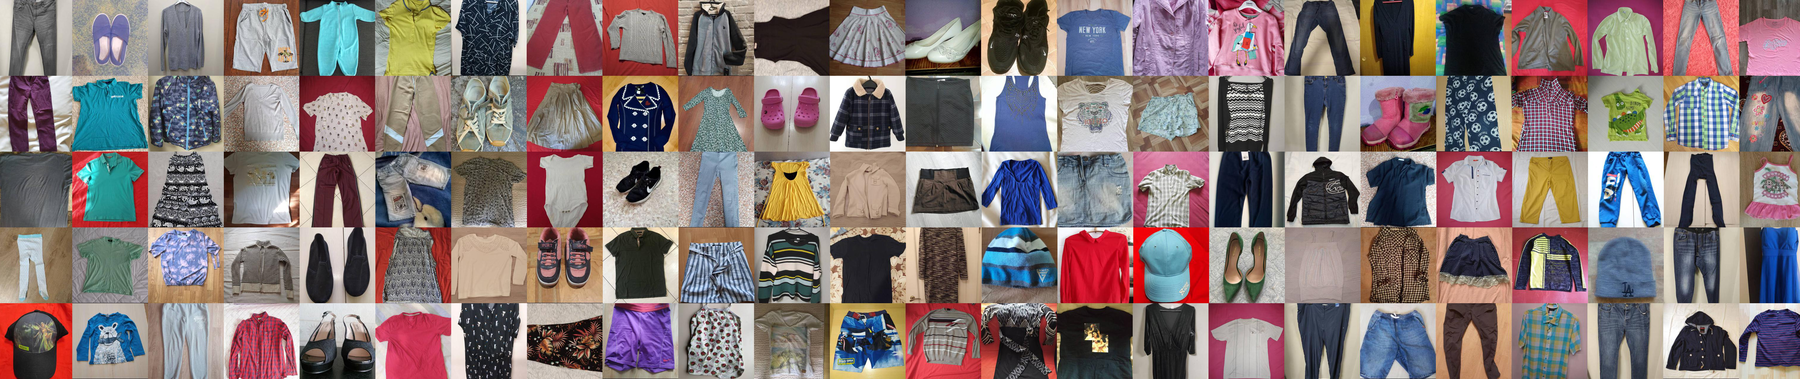
\includegraphics[scale = 0.25]{fileanh/44.png}
     \end{figure}
\end{center}

\subsubsection{Apparel images dataset}
\begin{itemize}
    \item Gồm có 11385 hình ảnh với các kích thước khác nhau.
    \item Độ lớn: 259MB
    \item Mô tả: Các hình ảnh được chia vào 1 trong 24 thư mục tùy thuộc vào mỗi loại và nàu sắc của đồ vật trong ảnh. Gồm hình ảnh về quần áo và giày.
    \item Được lấy trên Kaggle: \href{https://www.kaggle.com/datasets/trolukovich/apparel-images-dataset}{https://www.kaggle.com/datasets/trolukovich/apparel-images-dataset}
\end{itemize}
\begin{center}
    \begin{figure}[!h]
        \centering
        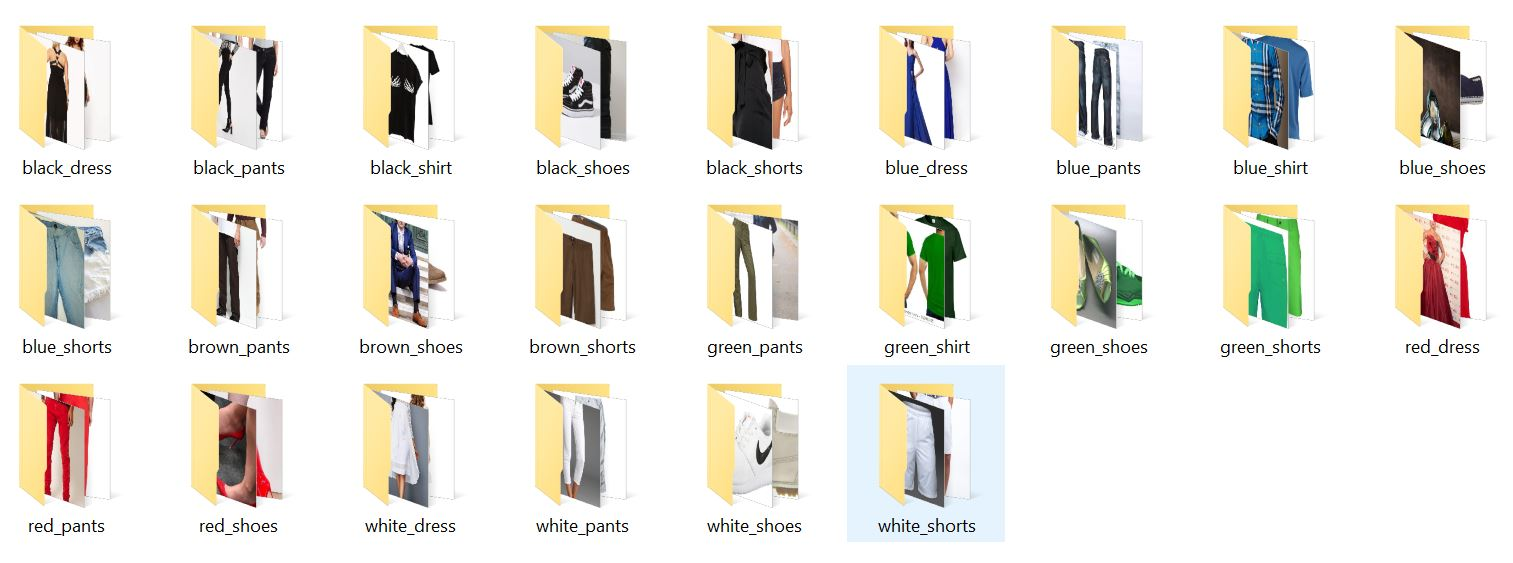
\includegraphics[scale = 0.45]{fileanh/45.jpg}
        \caption{Apparel images dataset}
    \end{figure}
\end{center}


\subsubsection{Shoe vs Sandal vs Boot Image Dataset}
\begin{itemize}
    \item Gồm có 15000 hình ảnh có độ phân giải 136x102 pixel trong mô hình màu RGB.
    \item Độ lớn: 47.4MB
    \item Mô tả: Bộ dữ liệu Hình ảnh Giày vs Sandal vs Boot này chứa 15.000 hình ảnh về giày, dép và bốt. 5000 hình ảnh cho mỗi thể loại. 
    \item Được lấy trên Kaggle: \href{https://www.kaggle.com/datasets/hasibalmuzdadid/shoe-vs-sandal-vs-boot-dataset-15k-images}{https://www.kaggle.com/datasets/hasibalmuzdadid/shoe-vs-sandal-vs-boot-dataset-15k-images}
\end{itemize}
\begin{center}
    \begin{figure}[!h]
        \centering
        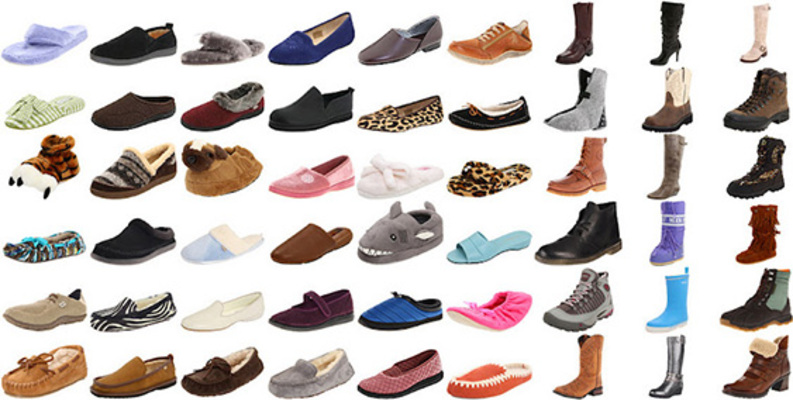
\includegraphics[scale = 1.5]{fileanh/46.jpg}
        \caption{Shoe Dataset}
    \end{figure}
\end{center}

\subsubsection{Một số nguồn dữ liệu khác được sử dụng}
\begin{enumerate}
    \item annotation Image Dataset : \href{https://universe.roboflow.com/honeysys/annotation-uzv7f/dataset/2}{https://universe.roboflow.com/honeysys/annotation-uzv7f/dataset/2}
    \begin{itemize}
        \item Có 2404 hình ảnh về nhẫn (phụ kiện) với cùng kích thước 640x640
        \item Độ lớn : 78.4MB
    \end{itemize}

    \item Bag Image Dataset: \href{https://universe.roboflow.com/bag-va5cg/bag-xbzrp/dataset/1}{https://universe.roboflow.com/bag-va5cg/bag-xbzrp/dataset/1}
    \begin{itemize}
        \item Có 1926 hình ảnh về túi xách (phụ kiện) với các kích thước khác nhau
        \item Độ lớn : 258MB
        
    \end{itemize}

    \item bucket-hats Image Dataset: \href{https://universe.roboflow.com/nathan-vdftz/bucket-hats/dataset/2}{https://universe.roboflow.com/nathan-vdftz/bucket-hats/dataset/2}
    \begin{itemize}
        \item Có 769 hình ảnh về mũ (phụ kiện) với các kích thước khác nhau
        \item Độ lớn : 21.2MB
      
    \end{itemize}

    \item yolo Image Dataset: \href{https://universe.roboflow.com/new-workspace-7lsw2/yolo-w9gld/dataset/2}{https://universe.roboflow.com/new-workspace-7lsw2/yolo-w9gld/dataset/2}
    \begin{itemize}
        \item Có 444 hình ảnh về mũ (phụ kiện) với với cùng kích thước 416x416
        \item Độ lớn : 4.48MB
      
    \end{itemize}
    
\end{enumerate}


\newpage
\subsection{Gán nhãn dữ liệu}
\subsubsection{Đổi tên cho hình ảnh}
Dưới đây là ví dụ cho tập dữ liệu Clothing dataset:
\begin{lstlisting}
for i, filename in enumerate(os.listdir(dataset_path)):
    i += 60001
    dst = f"{str(i)}.jpg"
    src =f"{dataset_path}{filename}"
    dst =f"{dataset_path}{dst}"
    os.rename(src, dst)
\end{lstlisting}
\begin{center}
    \begin{figure}[!h]
        \centering
        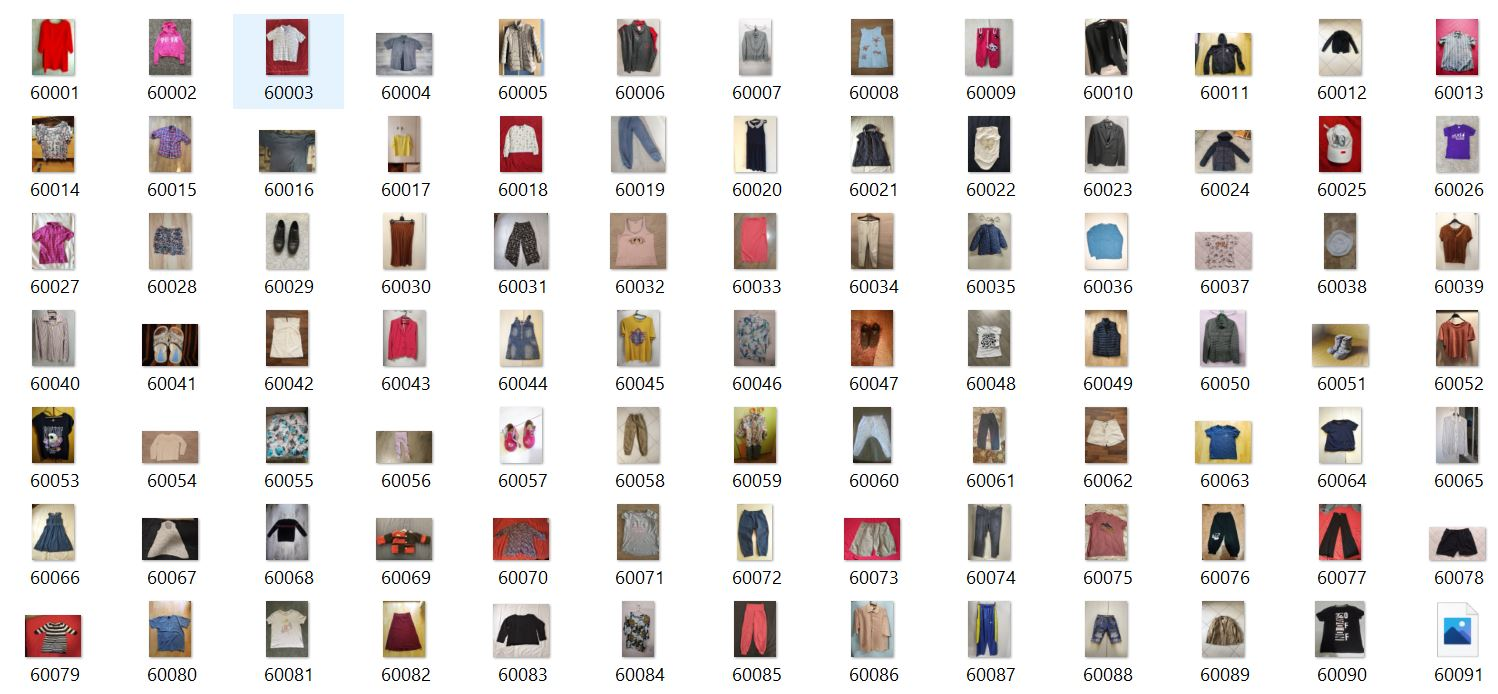
\includegraphics[scale = 0.6]{fileanh/47.jpg}
        \caption{Clothing dataset được đổi tên}
    \end{figure}
\end{center}
\begin{cy}
Các bộ dữ liệu khác làm tương tự.
\end{cy}


\subsubsection{Tạo nhãn cho từng bộ dữ liệu}
Do bộ dữ liệu \textbf{Clothing dataset} chứa tất cả hình ảnh của 3 lớp trong cùng 1 thư mục nên trước khi tạo nhãn ta sẽ phân chúng thành 3 thư mục và thực hiện đoạn code sau:
\begin{lstlisting}
app_path = 'C:/Users/admin/3D Objects/KhaiphaDL_CK/Models/images_compressed/Apparel/'
app = []
for img in os.listdir(app_path):   
    app.append([int(img[:5]), 'Apparel', img])
    
df_app = pd.DataFrame(app, columns = col_names)

acc_path = 'C:/Users/admin/3D Objects/KhaiphaDL_CK/Models/images_compressed/Accessories/'
acc = []
for img in os.listdir(acc_path):   
    acc.append([int(img[:5]), 'Accessories', img])
    
df_acc = pd.DataFrame(acc, columns = col_names)

foot_path = 'C:/Users/admin/3D Objects/KhaiphaDL_CK/Models/images_compressed/Footwear/'
foot = []
for img in os.listdir(foot_path):   
    foot.append([int(img[:5]), 'Footwear', img])
    
df_foot = pd.DataFrame(foot, columns = col_names)

df_app = df_app.append(df_acc,ignore_index = True)
df_app = df_app.append(df_foot,ignore_index = True)
df_app
\end{lstlisting}
\begin{center}
    \begin{figure}[!h]
        \centering
        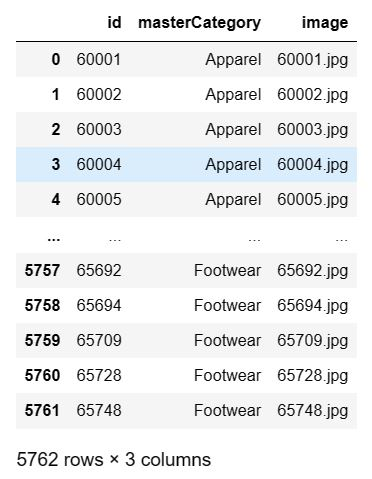
\includegraphics[scale = 1.4]{fileanh/48.jpg}
        \caption{Nhãn của Clothing dataset}
    \end{figure}
\end{center}
\begin{cy}
Các bộ dữ liệu còn lại đều đã được phân lớp thành các thư mục khác nhau hoặc chỉ có 1 lớp duy nhất nên sẽ chỉ cần tạo nhãn theo đúng thư mục tương ứng với lớp của nó.
\end{cy}
\newpage
\subsubsection{Tổng hợp dữ liệu}
\begin{enumerate}
    \item Hình ảnh: thực hiện chuyển hình ảnh của tất cả các bộ dữ liệu về thư mục './myntradataset/images' (thư mục chứa dữ liệu gốc được xử lý phía trên)

    \item Nhãn: Thực hiện tổng hợp lại nhãn của tất cả bộ dữ liệu cả gốc (\textbf{Fashion Product Images (Small)})và tăng cường thêm.
\end{enumerate}

\begin{center}
    \begin{figure}[!h]
        \centering
        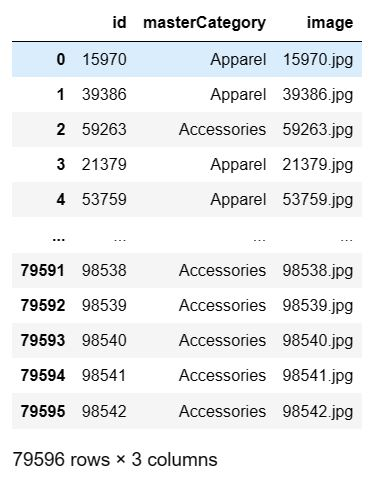
\includegraphics[scale = 1.4]{fileanh/49.jpg}
        \caption{Nhãn cho dữ liệu sau khi tăng cường}
    \end{figure}
\end{center}

\subsubsection{Kết quả thu được }
\begin{lstlisting}[language = python]
df_main['masterCategory'].value_counts()
\end{lstlisting}
Apparel    \ \ \ \ \ \ \ \ \ \ 34452\\
Accessories \   17033\\
Footwear    \ \ \ \ \ \  28111\\
Name: type, dtype: int64
\newpage
\begin{center}
    \begin{figure}[!h]
        \centering
        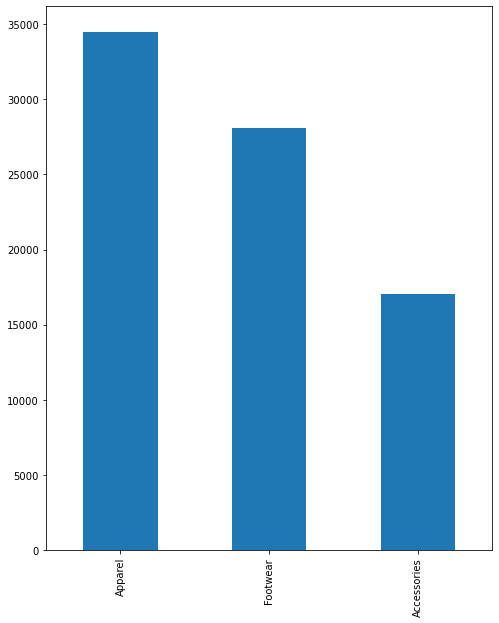
\includegraphics[scale = 0.6]{fileanh/50.png}
        \caption{Số lượng mỗi lớp sau khi tăng cường}
    \end{figure}
\end{center}

\begin{block}{Nhận xét}
Bài toán hiện tại sẽ gồm có:
\begin{itemize}
    \item 79596 hình ảnh đã được gán nhãn 
    \item 3 lớp chính với số lượng như sau:
    \begin{itemize}
        \item Apparel \ \ \ \ \ \ \ 34452
        \item Accessories \ \ 17033
        \item Footwear \ \ \ \ \ \ \ 28111
    \end{itemize}
\end{itemize}
\end{block}